\section{Sistemas de proyección}
\label{sec:cap2-sistemas-de-proyeccion}
Durante el siglo XVII, cartógrafos especializados, como Mercator, demostraron que no sólo el uso de
un sistema de proyección matemático y un ajustado sistema de coordenadas mejoraba la fiabilidad de
las medidas y la localización de las áreas de tierra, sino que el registro de fenómenos espaciales
a través de un modelo convenido de distribución de fenómenos naturales y asentamientos humanos era
de un valor incalculable para la navegación, para la búsqueda de rutas y en la estrategia militar
\citep{llopis2006sistemas}.

\subsection{Coordenadas geográficas}
Las coordenadas geográficas proveen un sistema de referencia, que se basan en la utilización de
coordenadas angulares como latitud y longitud (\figref{fig:sig-plano}). Su objetivo es el de
determinar los ángulos laterales de la superficie terrestre. Se denomina latitud al ángulo que
existe entre un punto cualquiera y el Ecuador, medida sobre el meridiano que pasa por dicho punto
\citep{fAlonsoSig2006}. La longitud mide el ángulo a lo largo de la línea del Ecuador desde
cualquier punto de la Tierra\citep{fAlonsoSig2006}.

\begin{figure}[!htbp]
\centering
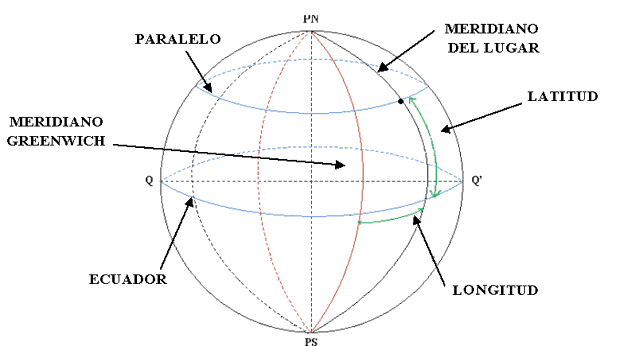
\includegraphics[width=0.7\textwidth]{capitulo-2/graphics/ejes-tierra.png}
\caption{\label{fig:sig-plano} Representación de los meridianos, paralelos, longitud y latitud en la superfice (Tomado de \cite{website:emcLonLat2014}).}
\end{figure}


Para la representación de objetos puntuales en una superficie, se utilizan las coordenadas $X$ e
$Y$ que caracterizan la planimetría y una coordenada $Z$ representa la altimertría del objeto
puntual en cuestión. En la \figref{fig:sig-xyz} se puede apreciar la representación de un objeto
puntual en una sistema tridimensional.

\begin{figure}[!htbp]
\centering
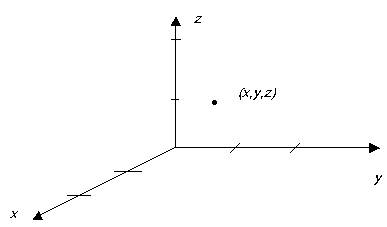
\includegraphics[width=0.5\textwidth]{capitulo-2/graphics/coordenadas-xyz.jpg}
\caption{\label{fig:sig-xyz} Representación de un objeto puntual en un sistema tridimensional
 $(x,y,z)$.}
\end{figure}

\subsection{Proyecciones}
Las proyecciones cartográficas o proyecciones geográficas se encuentran descritas por el conjunto
de métodos utilizados para establecer una correspondencia matemática entre los puntos pertenecientes a la superficie curva de la tierra y sus transformaciones en una superficie plana.

El problema principal a la hora de realizar una proyección es que no existe forma de representar
una superficie plana toda la superficie curva, de la tierra, sin deformarla siendo el objetivo
principal minimizar las deformaciones en la medida que sea posible \citep{fAlonsoSig2006}.
Teniendo en cuenta que la curvatura de la superficie terrestre es proporcional al tamaño del área
representada \citep{llopis2006sistemas}, si el área o región que se desea representar es pequeña,
entonces la deformación o distorsión resultante es despreciable, por lo que puede ser modelada con
coordenadas planas.

Con la aparición y difusión de los SIG, el conjunto de herramientas que ofrece se dio paso a
posibilidad de combinar información de diferentes mapas con diferentes proyecciones, esto ha
incrementado la relevancia de la cartografía más allá de la simple confección de mapas
\citep{llopis2006sistemas}.

\subsection{Elementos de representación cartográfica}
La representación de los objetos, recursos o fenómenos geográficos en una superficie o mapa, se
debe identificar los rasgos característicos teniendo en cuenta, principalmente, tres aspectos:
sus dimensiones, el nivel de medida y la distribución \citep{fomentoConceptos2010}. El análisis de
las características de estos elementos permiten seleccionar, adecuadamente, los símbolos a
utilizar para representar los fenómenos geográficos correspondientes \citep{fomentoConceptos2010}.
A cada entidad espacial puede ser asociada a diversas variables, para representar estas entidades
como hechos de la superficie terrestre, se han desarrollado un amplio conjunto de técnicas para
cartografiarlos.

\subsubsection{Dimensiones}
Teniendo en cuenta sus dimensiones y extensión, los fenómenos geográficos a ser representados en el
mapa pueden clasificarse en : puntuales, lineales, poligonales y espacio temporales
\citep{fAlonsoSig2006}.

\begin{itemize}
    \item \textit{Fenómenos puntuales} : indican la presencia de entidades de un modo puntual. Normalmente se utilizan se utilizan símbolos o colores para una variable cualitativa y distintos tamaños para las variables cuantitativas.

    \item \textit{Fenómenos lineales} : representan entidades naturales o artificiales de forma lineal, se encuentran conformadas a partir de dos o más fenómenos puntuales. Se pueden variar el ancho de de las líneas para describir la anchura de los elementos, también se utilizan distintos tipos de líneas (continuas y discontinuas) para caracterizar los fenómenos lineales.

    \item \textit{Fenómenos Poligonales} : Este fenómeno puede ser descrito por dos tipos de información bidimensional o tridimensional. Teniendo en cuenta el tamaño de los mismos pueden ser representados como polígonos o porciones homogéneas del terreno relacionadas a una variable cualitativa.

    \item \textit{Fenómenos espacio-temporales}: Existe una dependencia del fenómeno con respecto al paso del tiempo.
\end{itemize}

\subsubsection{Nivel de medida}

Los elementos de la naturaleza se miden con el fin de clarificarlos y, posteriormente, compararlos.
Esto no necesariamente implica a una magnitud cuantitativa, ya que pueden ser de utilizadas las
cualitativas u jerárquicas\citep{fomentoConceptos2010}. Teniendo en cuenta su orden de precisión
tenemos las siguientes escalas:

\begin{itemize}
    \item \textit{Nominal} : Se encarga de asignar una característica, no numérica, al fenómeno de forma que solo se pueden realizar comparaciones cualitativas. Este es el nivel más elemental de medida, pues no informa acerca de la cantidad o el orden.

    \item \textit{Ordinal} : Se establece una jerarquía no cuantificable entre los diferentes elementos. Por ejemplo, un mapa en el que aparecen núcleos de población, cuyos símbolos están jerarquizados según el número de habitantes sin especificar cantidad.

    \item \textit{Cuantitativa} :Asigna una característica numérica a un fenómeno geográfico, normalmente es necesario emplear algún tipo de unidad convencional.
\end{itemize}

\subsubsection{Distribución}
La distribución de los fenómenos, o su ocurrencia, puede darse a lo largo y ancho de la superficie
terrestre que los alberga ya sea de forma continua en una ubicación de la superficie o de forma
discontinua \citep{fomentoConceptos2010}. Estos fenómenos pueden dividirse, de acuerdo a su distribución, en :

\begin{itemize}
    \item \textit{Continuos} : Son aquellos que tienen presencia en todos los puntos de la superficie, aunque sólo se cuenten con las medidas de algunos puntos significativos de la superficie. En esta categoría tenemos a la temperatura y la densidad poblacional.

    \item \textit{Discretos} : son aquellos fenómenos que tiene presencia sólo en algunos puntos de la superficie. Algunos de estos fenómenos discretos pueden transformarse en continuos mediante la aplicación de una relación. Por ejemplo tenemos el fenómeno discreto, número de habitantes de una provincia, para que se transforme en un fenómeno continuo se debe dividir el número de habitantes con el tamaño de la superficie en $km^2$, de esta forma podemos obtener la densidad poblacional que es un fenómeno continuo.
\end{itemize}
